\chapter{Pericyclic Reactions}\label{ch:b3:pericyclic}

Sunlight falling on skin opens a ring of 7-dehydrocholesterol in a fraction
of a second; body heat then moves one hydrogen atom across seven carbon atoms,
and the product is vitamin D$_3$. Neither step has an intermediate: bonds break
and form together, around a ring of atoms, along a single transition state. The
first step goes only with light and the second only with heat, and each gives
one stereoisomer. This chapter explains why, from the symmetry of the
molecular orbitals involved: the rules found by Robert Woodward and Roald
Hoffmann, which predict whether such a reaction can happen and what it gives.

\begin{recall}
The Year 2 volume gave the Hückel coefficients of polyenes, aromatic and
antiaromatic rings, HOMO, LUMO and frontier orbitals, concerted reactions, and
the Diels--Alder reaction of a diene with a dienophile with its endo rule; the
Year 1 volume \textit{Z}/\textit{E} descriptors. \Cref{ch:b3:point-groups} defined the $C_2$ axis
and the \omterm{def:b3:point-groups:mirror}{mirror plane}, \cref{ch:b3:photochemistry} excited states and the [2+2]
photocycloaddition.
\end{recall}

\begin{omfigure}
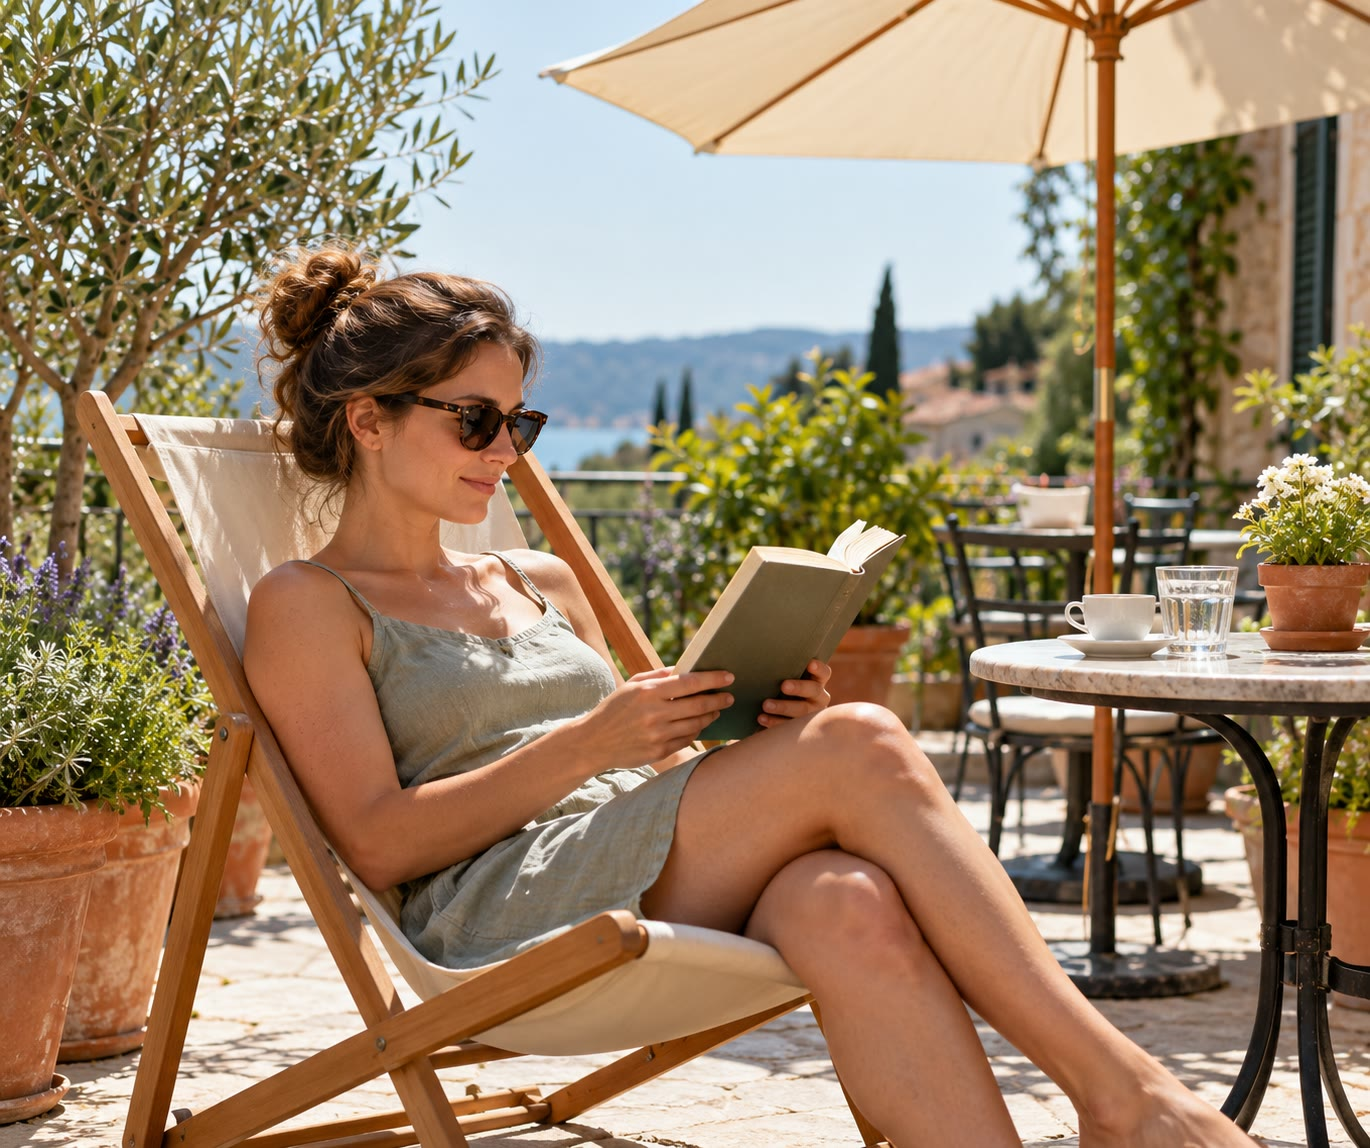
\includegraphics[width=0.55\linewidth]{images/book4/ai/b3-26-terrace.jpg}

{\small Reading on a sunny terrace: ultraviolet light reaching the skin starts
the synthesis of vitamin D$_3$ with a pericyclic ring opening.}
\end{omfigure}

\section{Four families}

\begin{definition}[Pericyclic reaction]\label{def:b3:pericyclic:pericyclic}
A \emph{pericyclic reaction}\index{pericyclic reaction} is a concerted reaction
whose transition state is a cyclic array of interacting orbitals, in which all
the bonds are made and broken around the ring at the same time.
\end{definition}

\begin{definition}[Families of pericyclic reactions]\label{def:b3:pericyclic:families}
In an \emph{electrocyclic reaction}\index{electrocyclic reaction} a conjugated
polyene closes into a ring by forming a $\sigma$ bond between its termini, or the
reverse. In a \emph{cycloaddition}\index{cycloaddition}, two $\pi$ systems join
into a ring by forming two $\sigma$ bonds; an $[m + n]$ cycloaddition joins components
of $m$ and $n$ atoms (or electrons). In a \emph{sigmatropic
rearrangement}\index{sigmatropic rearrangement} a $\sigma$ bond migrates along a $\pi$
system; in an $[i, j]$ shift the bond moves from atoms 1 and 1 to atoms $i$ and $j$
of the two fragments. A \emph{cheletropic reaction}\index{cheletropic reaction}
makes or breaks two bonds to the same atom, as when sulfur dioxide
leaves a sulfolene. In an \emph{ene reaction}\index{ene reaction} an alkene
with an allylic hydrogen adds to a $\pi$ bond, the hydrogen moving with it.
\end{definition}

\begin{definition}[Suprafacial and antarafacial]\label{def:b3:pericyclic:faciality}
A component reacts \emph{suprafacially}\index{suprafacial} when its two new
bonds form, or its two old ones break, on the same face of its $\pi$ system (or with
retention at a $\sigma$ bond), and \emph{antarafacially}\index{antarafacial} when they
are on opposite faces (or with inversion).
\end{definition}

\section{Electrocyclic reactions}

\begin{definition}[Conrotatory and disrotatory]\label{def:b3:pericyclic:rotation-modes}
In an electrocyclic ring closure the two terminal groups rotate about the bonds
that join them to the chain. The rotation is \emph{conrotatory}\index{conrotatory}
when both turn in the same sense (both clockwise seen along the chain), and
\emph{disrotatory}\index{disrotatory} when they turn in opposite senses.
\end{definition}

\begin{theorem}[Electrocyclic reactions]\label{thm:b3:pericyclic:electrocyclic}
A thermal \omterm{def:b3:pericyclic:families}{electrocyclic reaction} of a polyene with $4n$ $\pi$ electrons is
\omterm{def:b3:pericyclic:rotation-modes}{conrotatory}, and with $4n + 2$ $\pi$ electrons \omterm{def:b3:pericyclic:rotation-modes}{disrotatory}.
\end{theorem}

\begin{proof}
The new $\sigma$ bond forms from the terminal p orbitals of the HOMO, which in the
thermal reaction holds the highest-energy electrons; it is bonding only if the
lobes that turn to face each other have the same sign. By the Hückel formula
(\cref{ch:b3:solid-state}) the coefficients of orbital $k$ of an $N$-atom chain are
proportional to $\sin(jk\pi/(N + 1))$, so the two termini, $j = 1$ and $j = N$, have
coefficients $\sin(k\pi/(N + 1))$ and $\sin(Nk\pi/(N + 1)) = (-1)^{k+1}\sin(k\pi/(N + 1))$: the same sign for odd $k$,
opposite signs for even $k$. With $N$ atoms and $N$ electrons the HOMO is
$k = N/2$. For $N = 4n$, $k = 2n$ is even: the upper lobes of the termini have opposite
signs, and the two termini must turn the same way, each bringing its lobe of
the matching sign inwards: \omterm{def:b3:pericyclic:rotation-modes}{conrotatory}. For $N = 4n + 2$, $k = 2n + 1$ is odd: the upper lobes
have the same sign, and turning them towards each other is \omterm{def:b3:pericyclic:rotation-modes}{disrotatory}.
\end{proof}

\begin{omfigure}
\begin{tikzpicture}[font=\small, >=Stealth]
  % butadiene HOMO psi2: 0.60 0.37 -0.37 -0.60 (lobes scaled x1.6)
  \foreach \x/\c in {0/0.60, 1/0.37, 2/-0.37, 3/-0.60} {
    \pic at (\x,0) {omp={1.6*\c}{90}};
    \fill (\x,0) circle (1.2pt);
  }
  \draw[black!60] (0,0) -- (3,0);
  \draw[->, thick, omThm] (-0.45,0.55) arc[start angle=130, end angle=20, radius=0.7];
  \draw[->, thick, omThm] (2.55,0.55) arc[start angle=130, end angle=20, radius=0.7];
  \node[font=\scriptsize, align=center] at (1.5,-1.3) {butadiene, $\psi_2$ (HOMO, 4 electrons):\\ termini of opposite sign: \textbf{conrotatory}};
  \begin{scope}[xshift=6.2cm]
  % hexatriene HOMO psi3: 0.52 0.23 -0.42 -0.42 0.23 0.52
  \foreach \x/\c in {0/0.52, 0.8/0.23, 1.6/-0.42, 2.4/-0.42, 3.2/0.23, 4.0/0.52} {
    \pic at (\x,0) {omp={1.6*\c}{90}};
    \fill (\x,0) circle (1.2pt);
  }
  \draw[black!60] (0,0) -- (4.0,0);
  \draw[->, thick, omThm] (-0.45,0.55) arc[start angle=130, end angle=20, radius=0.7];
  \draw[->, thick, omThm] (4.45,0.55) arc[start angle=50, end angle=160, radius=0.7];
  \node[font=\scriptsize, align=center] at (2.0,-1.3) {hexatriene, $\psi_3$ (HOMO, 6 electrons):\\ termini of the same sign: \textbf{disrotatory}};
  \end{scope}
\end{tikzpicture}

{\small The HOMO of butadiene and of hexatriene, with lobes scaled by their
Hückel coefficients (blue and orange: the two signs), drawn along the chain.
For a bond to form between the termini, the lobes that turn to face each other
must have the same sign: both termini turn clockwise in butadiene, in opposite
senses in hexatriene (red arrows).}
\end{omfigure}

The rule is stereospecific. (\textit{E},\textit{E})-hexa-2,4-diene, heated, would close
conrotatorily into \textit{trans}-3,4-dimethylcyclobutene; in practice the strained
cyclobutene is the one that opens, and \textit{cis}-3,4-dimethylcyclobutene opens
conrotatorily into (\textit{E},\textit{Z})-hexa-2,4-diene only. (\textit{E},\textit{Z},\textit{E})-octa-2,4,6-triene closes
disrotatorily into \textit{cis}-5,6-dimethylcyclohexa-1,3-diene.

\begin{proposition}[Photochemical electrocyclic reactions]\label{prop:b3:pericyclic:photo-electrocyclic}
Under light the rules are reversed: $4n$ electrons, \omterm{def:b3:pericyclic:rotation-modes}{disrotatory}; $4n + 2$, \omterm{def:b3:pericyclic:rotation-modes}{conrotatory}.
\end{proposition}

\begin{proof}
Absorbing a photon promotes an electron from the HOMO $k = N/2$ to the LUMO $k = N/2 + 1$
(\cref{ch:b3:photochemistry}), which is now the highest occupied orbital and
controls the termini. Its $k$ has the opposite parity, so the relative sign of its
terminal coefficients is reversed, and with it the sense of rotation.
\end{proof}

\begin{method}[Predicting the stereochemistry of an electrocyclic reaction]\label{met:b3:pericyclic:predict-stereo}
\begin{enumerate}
  \item Count the $\pi$ electrons of the open-chain polyene ($4n$ or $4n + 2$); note heat or
        light.
  \item Read the mode: thermal $4n$ con, $4n + 2$ dis; photochemical reversed.
  \item Draw the termini with their substituents, in the conformation that
        closes (s-cis); turn them by 90° in the chosen mode.
  \item Read whether the two substituents end on the same face of the ring
        (\textit{cis}) or on opposite faces (\textit{trans}). For a ring opening, run the same
        analysis backwards.
\end{enumerate}
\end{method}

\section{Orbital correlation diagrams}

Woodward and Hoffmann's original argument looks at all the orbitals, not only
the HOMO. Along a \omterm{def:b3:pericyclic:rotation-modes}{conrotatory} path the molecule keeps a $C_2$ axis; along a
\omterm{def:b3:pericyclic:rotation-modes}{disrotatory} path, a \omterm{def:b3:point-groups:mirror}{mirror plane} $\sigma$. Each orbital of the reactant and of the
product is symmetric (S) or antisymmetric (A) with respect to the element that
is kept.

\begin{definition}[Orbital correlation diagram]\label{def:b3:pericyclic:orbital-correlation}
An \emph{orbital correlation diagram}\index{orbital correlation diagram} links
each orbital of the reactant to the orbital of the product of the same symmetry,
with respect to the \omterm{def:b3:point-groups:operation}{symmetry elements} kept along the reaction path, taking them
in order of energy: the lowest S with the lowest S, and so on.
\end{definition}

\begin{proposition}[Conservation of orbital symmetry]\label{prop:b3:pericyclic:correlation}
If every orbital occupied in the reactant correlates with an orbital occupied in
the product, the thermal reaction is allowed; if an occupied orbital correlates
with an empty one, it is forbidden, with a high barrier.
\end{proposition}

\begin{proof}[Argued]
Along the path, an orbital keeps its symmetry and its energy changes
continuously; orbitals of the same symmetry cannot cross (they mix and repel),
those of different symmetry can. When a doubly occupied orbital of the reactant
must become an antibonding orbital of the product, the ground state of the
reactant leads to a doubly excited state of the product, and the ground-state
energy rises steeply until, late on the path, the states of the same symmetry
mix: the barrier is high.
\end{proof}

\begin{omfigure}
\begin{tikzpicture}[font=\scriptsize]
  \foreach \px/\title/\el in {0/disrotatory: $\sigma$ kept/s, 7.6/conrotatory: $C_2$ kept/c} {
    \begin{scope}[xshift=\px cm]
    \node[font=\small\bfseries] at (2.0,5.1) {\title};
    \node at (0,4.7) {butadiene};
    \node at (4.0,4.7) {cyclobutene};
    \end{scope}
  }
  % ---- disrotatory (mirror): butadiene psi1 S, psi2 A, psi3 S, psi4 A;
  %      cyclobutene sigma S, pi S, pi* A, sigma* A
  \pic (b1) at (0,0.6) {omlevel={ud}{1.0}}; \node[anchor=east] at (-0.6,0.6) {$\psi_1$ S};
  \pic (b2) at (0,1.8) {omlevel={ud}{1.0}}; \node[anchor=east] at (-0.6,1.8) {$\psi_2$ A};
  \pic (b3) at (0,3.0) {omlevel={}{1.0}}; \node[anchor=east] at (-0.6,3.0) {$\psi_3$ S};
  \pic (b4) at (0,4.1) {omlevel={}{1.0}}; \node[anchor=east] at (-0.6,4.1) {$\psi_4$ A};
  \pic (c1) at (4.0,0.1) {omlevel={ud}{1.0}}; \node[anchor=west] at (4.6,0.1) {$\sigma$ S};
  \pic (c2) at (4.0,1.3) {omlevel={ud}{1.0}}; \node[anchor=west] at (4.6,1.3) {$\pi$ S};
  \pic (c3) at (4.0,3.4) {omlevel={}{1.0}}; \node[anchor=west] at (4.6,3.4) {$\pi^*$ A};
  \pic (c4) at (4.0,4.4) {omlevel={}{1.0}}; \node[anchor=west] at (4.6,4.4) {$\sigma^*$ A};
  \draw[omcorr] (b1-r) -- (c1-l);
  \draw[omcorrforbidden] (b2-r) -- (c3-l);
  \draw[omcorr] (b3-r) -- (c2-l);
  \draw[omcorr] (b4-r) -- (c4-l);
  % ---- conrotatory (C2): butadiene psi1 A, psi2 S, psi3 A, psi4 S;
  %      cyclobutene sigma S, pi A, pi* S, sigma* A
  \begin{scope}[xshift=7.6cm]
  \pic (d1) at (0,0.6) {omlevel={ud}{1.0}}; \node[anchor=east] at (-0.6,0.6) {$\psi_1$ A};
  \pic (d2) at (0,1.8) {omlevel={ud}{1.0}}; \node[anchor=east] at (-0.6,1.8) {$\psi_2$ S};
  \pic (d3) at (0,3.0) {omlevel={}{1.0}}; \node[anchor=east] at (-0.6,3.0) {$\psi_3$ A};
  \pic (d4) at (0,4.1) {omlevel={}{1.0}}; \node[anchor=east] at (-0.6,4.1) {$\psi_4$ S};
  \pic (e1) at (4.0,0.1) {omlevel={ud}{1.0}}; \node[anchor=west] at (4.6,0.1) {$\sigma$ S};
  \pic (e2) at (4.0,1.3) {omlevel={ud}{1.0}}; \node[anchor=west] at (4.6,1.3) {$\pi$ A};
  \pic (e3) at (4.0,3.4) {omlevel={}{1.0}}; \node[anchor=west] at (4.6,3.4) {$\pi^*$ S};
  \pic (e4) at (4.0,4.4) {omlevel={}{1.0}}; \node[anchor=west] at (4.6,4.4) {$\sigma^*$ A};
  \draw[omcorr] (d1-r) -- (e2-l);
  \draw[omcorr] (d2-r) -- (e1-l);
  \draw[omcorr] (d3-r) -- (e4-l);
  \draw[omcorr] (d4-r) -- (e3-l);
  \end{scope}
\end{tikzpicture}

{\small \omterm{def:b3:pericyclic:orbital-correlation}{Orbital correlation diagrams} for butadiene $\rightleftharpoons$ cyclobutene. Left, the
\omterm{def:b3:pericyclic:rotation-modes}{disrotatory} path keeps a \omterm{def:b3:point-groups:mirror}{mirror plane}: the occupied $\psi_2$ (A) correlates with the
empty $\pi^*$ (A) of cyclobutene (red dashed): thermally forbidden. Right, the
\omterm{def:b3:pericyclic:rotation-modes}{conrotatory} path keeps a $C_2$ axis: occupied orbitals go to occupied orbitals:
thermally allowed.}
\end{omfigure}

\begin{method}[Building a correlation diagram]\label{met:b3:pericyclic:correlation-diagram}
\begin{enumerate}
  \item Find the \omterm{def:b3:point-groups:operation}{symmetry elements} that bisect the bonds made and broken and are
        kept all along the chosen path.
  \item List the orbitals taking part, of reactant and product, in order of
        energy, and label each S or A for each element.
  \item Join the lowest orbital of each symmetry type on one side to the lowest of
        the same type on the other, then the next, never crossing two lines of the
        same symmetry.
  \item Check the occupied orbitals: all to occupied, allowed; one to empty,
        forbidden.
\end{enumerate}
\end{method}

\begin{definition}[State correlation diagram]\label{def:b3:pericyclic:state-correlation}
A \emph{state correlation diagram}\index{state correlation diagram} links the
electronic states of reactant and product, each built from the orbital
configurations and labelled by its overall symmetry, through the path; states of
the same symmetry do not cross.
\end{definition}

For the forbidden \omterm{def:b3:pericyclic:rotation-modes}{disrotatory} path, the ground state of butadiene ($\psi_1^2\psi_2^2$)
correlates with a doubly excited state of cyclobutene ($\sigma^2\pi^{*2}$), but the first excited
state ($\psi_1^2\psi_2\psi_3$) correlates with the first excited state of cyclobutene ($\sigma^2\pi\pi^*$): from the
excited state, the \omterm{def:b3:pericyclic:rotation-modes}{disrotatory} path is downhill. That is the photochemical
reversal of \cref{prop:b3:pericyclic:photo-electrocyclic}, seen on the states.

\section{Cycloadditions}

\begin{theorem}[Cycloadditions]\label{thm:b3:pericyclic:cycloaddition}
A thermal $[m + n]$ \omterm{def:b3:pericyclic:families}{cycloaddition} in which both components react \omterm{def:b3:pericyclic:faciality}{suprafacially} is
allowed when $m + n = 4q + 2$ electrons, and forbidden when $m + n = 4q$; under light the
rule is reversed.
\end{theorem}

\begin{proof}
Both new bonds form between the HOMO of one component and the LUMO of the
other, which face each other with their terminal lobes; with both reacting
\omterm{def:b3:pericyclic:faciality}{suprafacially}, both bonds are bonding only if the terminal coefficients of the
HOMO and of the LUMO have the same relative sign. For a component of $N$
electrons on $N$ atoms, the HOMO has $k = N/2$ and the LUMO $k = N/2 + 1$; terminal coefficients of the
same sign for odd $k$, opposite for even $k$. In the [4+2] case, the diene HOMO ($k = 2$)
and the ethene LUMO ($k = 2$) both have opposite terminal signs: they match. In the
[2+2] case, the HOMO of one ethene ($k = 1$, same signs) meets the LUMO of the other
($k = 2$, opposite): one end bonding, one antibonding. In general the HOMO of the $m$
component and the LUMO of the $n$ component match when $m/2$ and $n/2 + 1$ have the same
parity, that is when $(m + n)/2$ is odd: $m + n = 4q + 2$. Under light, the singly occupied LUMO of
the excited component plays the part of its HOMO, and the parity condition is
reversed.
\end{proof}

\begin{omfigure}
\begin{tikzpicture}[font=\scriptsize]
  % [4+2]: diene HOMO above, ethene LUMO (pi*) below, facing lobes match at both ends
  \foreach \x/\c in {0/0.60, 1/0.37, 2/-0.37, 3/-0.60} {
    \pic at (\x,1.6) {omp={1.4*\c}{90}}; \fill (\x,1.6) circle (1.1pt);
  }
  \draw[black!60] (0,1.6) -- (3,1.6);
  \foreach \x/\c in {0/-0.71, 3/0.71} {
    \pic at (\x,-0.4) {omp={1.4*\c}{90}}; \fill (\x,-0.4) circle (1.1pt);
  }
  \draw[black!60] (0,-0.4) -- (3,-0.4);
  \draw[omMeth, densely dashed, thick] (-0.25,0.75) -- (-0.25,0.35) (3.25,0.75) -- (3.25,0.35);
  \node[omMeth] at (-0.25,0.55) [left] {bonding};
  \node[omMeth] at (3.25,0.55) [right] {bonding};
  \node[font=\small] at (1.5,2.95) {[4+2]: diene HOMO};
  \node[font=\small] at (1.5,-1.75) {ethene LUMO: allowed};
  \begin{scope}[xshift=7.2cm]
  \foreach \x/\c in {0/0.71, 3/0.71} {
    \pic at (\x,1.6) {omp={1.4*\c}{90}}; \fill (\x,1.6) circle (1.1pt);
  }
  \draw[black!60] (0,1.6) -- (3,1.6);
  \foreach \x/\c in {0/-0.71, 3/0.71} {
    \pic at (\x,-0.4) {omp={1.4*\c}{90}}; \fill (\x,-0.4) circle (1.1pt);
  }
  \draw[black!60] (0,-0.4) -- (3,-0.4);
  \draw[omMeth, densely dashed, thick] (-0.25,0.75) -- (-0.25,0.35);
  \draw[omThm, densely dashed, thick] (3.25,0.75) -- (3.25,0.35);
  \node[omMeth] at (-0.25,0.55) [left] {bonding};
  \node[omThm] at (3.25,0.55) [right] {antibonding};
  \node[font=\small] at (1.5,2.95) {[2+2]: ethene HOMO};
  \node[font=\small] at (1.5,-1.75) {ethene LUMO: forbidden};
  \end{scope}
\end{tikzpicture}

{\small Frontier orbitals facing each other in \omterm{def:b3:pericyclic:faciality}{suprafacial} \omterm{def:b3:pericyclic:families}{cycloadditions} (the
lower lobes of the upper component meet the upper lobes of the lower one; lobe
sizes from the Hückel coefficients). In the [4+2] reaction both new bonds are
bonding; in the [2+2] reaction one end is bonding and the other antibonding.}
\end{omfigure}

Thermally, two alkenes do not give a cyclobutane in one concerted step; under
light they do (\cref{ch:b3:photochemistry}). Ketenes are the exception that
proves the rule: their C=O $\pi^*$ orbital, perpendicular to the C=C one, lets them
react with an alkene in a [$\pi2_s$ + $\pi2_a$] geometry, one component \omterm{def:b3:pericyclic:faciality}{suprafacial} and the
ketene \omterm{def:b3:pericyclic:faciality}{antarafacial}, and they form cyclobutanones thermally.

\begin{definition}[1,3-Dipolar cycloadditions]\label{def:b3:pericyclic:dipolar}
A \emph{1,3-dipole}\index{1,3-dipole} is a three-atom $\pi$ system with four
electrons, written with formal charges at its ends or in the middle, such as an
azide $\ce{R-N=N+=N-}$, a nitrile oxide or an ozone molecule. A \emph{1,3-dipolar
cycloaddition}\index{1,3-dipolar cycloaddition} is its [3+2] \omterm{def:b3:pericyclic:families}{cycloaddition}, a
six-electron reaction, with an alkene or alkyne, giving a five-membered ring.
\end{definition}

The copper-catalysed reaction of an azide with a terminal alkyne, giving one
regioisomer of a 1,2,3-triazole, is the reliable joining reaction of click
chemistry. Ozonolysis starts with a \omterm{def:b3:pericyclic:dipolar}{1,3-dipolar cycloaddition} of ozone to the
alkene.

\section{Sigmatropic rearrangements and the general rule}

\begin{proposition}[Hydrogen shifts]\label{prop:b3:pericyclic:sigmatropic-h}
A thermal $[1, j]$ shift of hydrogen along a polyene is allowed \omterm{def:b3:pericyclic:faciality}{suprafacially} when the
transition state holds $4q + 2$ electrons ($[1,5]$) and must be \omterm{def:b3:pericyclic:faciality}{antarafacial} when it holds $4q$
($[1,3]$, $[1,7]$).
\end{proposition}

\begin{proof}
Treat the transition state as a hydrogen atom (1s) moving between the ends of a
radical of $j$ atoms with $j$ electrons; the hydrogen bridges the two termini of the
SOMO, $k = (j + 1)/2$. For $j = 5$, $k = 3$ is odd, the termini have lobes of the same sign on one face,
and the 1s orbital can bond to both on that face: \omterm{def:b3:pericyclic:faciality}{suprafacial}. For $j = 3$ and $j = 7$,
$k = 2$ and $4$ are even, the same-sign lobes are on opposite faces at the two ends, and
the hydrogen must pass from one face to the other: \omterm{def:b3:pericyclic:faciality}{antarafacial}. A $[1,3]$ shift
cannot reach across so short a chain; a $[1,7]$ shift can, along a helical polyene.
\end{proof}

\begin{definition}[Cope and Claisen rearrangements]\label{def:b3:pericyclic:cope-claisen}
The \emph{Cope rearrangement}\index{Cope rearrangement} is the [3,3] \omterm{def:b3:pericyclic:families}{sigmatropic rearrangement}
of a hexa-1,5-diene; the \emph{Claisen
rearrangement}\index{Claisen rearrangement} that of an allyl vinyl ether, or of
an allyl aryl ether, into a $\gamma,\delta$-unsaturated carbonyl compound or an \textit{ortho}-allylphenol.
\end{definition}

\begin{omfigure}
\begin{tikzpicture}[font=\scriptsize, scale=1.1]
  \foreach \px/\three/\title in {0/C/Cope, 5.0/O/Claisen} {
    \begin{scope}[xshift=\px cm]
      % chair: atoms at 60-degree steps, alternately 0.25 above and below the
      % mean plane, seen from slightly above (y' = 0.35 y + z), scaled
      \begin{scope}[shift={(1.3,0.2)}, scale=1.15]
      \coordinate (a1) at (-1.25,-0.25); \coordinate (a2) at (-0.625,-0.129); \coordinate (a3) at (0.625,-0.629);
      \coordinate (a4) at (1.25,0.25); \coordinate (a5) at (0.625,0.129); \coordinate (a6) at (-0.625,0.629);
      \end{scope}
      \draw[thick] (a1) -- (a2) -- (a3);
      \draw[thick] (a4) -- (a5) -- (a6);
      \draw[omThm, thick, densely dashed] (a3) -- (a4);
      \draw[omMeth, thick, densely dashed] (a6) -- (a1);
      \foreach \i/\l in {1/1, 2/2, 4/4, 5/5, 6/6} { \fill (a\i) circle (1.3pt); }
      \node[fill=white, inner sep=0.6pt] at (a3) {\three};
      \node[anchor=east] at (a1) {1};
      \node[anchor=north] at (a2) {2};
      \node[anchor=north west] at (a3) {3};
      \node[anchor=west] at (a4) {4};
      \node[anchor=south] at (a5) {5};
      \node[anchor=south] at (a6) {6};
      \node[font=\small\bfseries] at (1.3,1.5) {\title};
    \end{scope}
  }
\end{tikzpicture}

{\small Chair transition states of [3,3] \omterm{def:b3:pericyclic:families}{sigmatropic rearrangements}: two allyl
fragments face each other; the 3--4 $\sigma$ bond breaks (red) while the 1--6 bond forms
(green). In the \omterm{def:b3:pericyclic:cope-claisen}{Claisen rearrangement} atom 3 is the ether oxygen, and the
product is a carbonyl compound. The chair fixes the relative configuration of
new stereocentres.}
\end{omfigure}

The [3,3] shift is a six-electron, \omterm{def:b3:pericyclic:faciality}{all-suprafacial} process, allowed thermally;
it runs through a chair-like transition state, like a cyclohexane, and
substituents prefer its equatorial positions: (\textit{E},\textit{E}) and (\textit{Z},\textit{Z}) dienes give
opposite relative configurations, predictably.

\begin{theorem}[Woodward--Hoffmann rules]\label{thm:b3:pericyclic:woodward-hoffmann}
A thermal \omterm{def:b3:pericyclic:pericyclic}{pericyclic reaction} is allowed when the total number of $(4q + 2)_s$ and
$(4r)_a$ components is odd; a photochemical one when it is even.
\end{theorem}

\begin{proof}[Partial proof]
For each family treated above the count agrees with the frontier-orbital
analysis: a thermal [4+2] \omterm{def:b3:pericyclic:families}{cycloaddition} has components $\pi4_s$ and $\pi2_s$, one $(4q + 2)_s$
component, odd: allowed; the [2+2] has $\pi2_s + \pi2_s$, two, even: forbidden, while
$\pi2_s + \pi2_a$ has one: allowed; the \omterm{def:b3:pericyclic:rotation-modes}{conrotatory} opening of cyclobutene is $\sigma2_s + \pi2_a$, one:
allowed; the \omterm{def:b3:pericyclic:faciality}{suprafacial} $[1,5]$-H shift is $\sigma2_s + \pi4_s$, where only $\sigma2_s$ counts: one,
allowed. The general proof, valid for every array of components, belongs
to more advanced courses.
\end{proof}

\begin{definition}[Aromatic and Möbius transition states]\label{def:b3:pericyclic:mobius}
An \emph{aromatic transition state}\index{aromatic transition state} is a cyclic
array of orbitals in a pericyclic transition state that, like a Hückel ring, is
stabilised when it holds $4q + 2$ electrons. A \emph{Möbius transition
state}\index{Möbius transition state} has an odd number of sign changes between
neighbouring orbitals around the ring (one \omterm{def:b3:pericyclic:faciality}{antarafacial} twist); it is
stabilised with $4q$ electrons.
\end{definition}

\begin{proposition}[Aromatic transition states]\label{prop:b3:pericyclic:aromatic-ts}
A thermal \omterm{def:b3:pericyclic:pericyclic}{pericyclic reaction} is allowed when its transition state is aromatic:
Hückel topology with $4q + 2$ electrons, or Möbius topology with $4q$ electrons.
\end{proposition}

\begin{proof}[Argued]
The cyclic array of orbitals in the transition state behaves like a cyclic
conjugated molecule. A Hückel ring has its lowest level non-degenerate and pairs
above it, filled with $4q + 2$ electrons (Year 2 volume); a ring with one sign
inversion has all its levels in pairs, filled with $4q$. A filled shell means
stabilisation, an \omterm{def:b3:pericyclic:mobius}{aromatic transition state} and a low barrier. The count of sign
changes is the count of \omterm{def:b3:pericyclic:faciality}{antarafacial} components, so this rule is equivalent to the
Woodward--Hoffmann rule.
\end{proof}

\begin{method}[Drawing and counting components]\label{met:b3:pericyclic:components}
\begin{enumerate}
  \item Mark the bonds made and broken; each $\pi$ system or $\sigma$ bond that changes is a
        component, labelled with its type and electron count ($\pi4$, $\pi2$, $\sigma2$, $\omega0$ for
        an empty orbital).
  \item Choose s or a for each component from the geometry (same face, or
        opposite faces).
  \item Count the $(4q + 2)_s$ and $(4r)_a$ components: odd, allowed thermally; even, allowed
        photochemically.
  \item Cross-check with the electron count around the ring: Hückel with $4q + 2$,
        Möbius with $4q$.
\end{enumerate}
\end{method}

\begin{omfigure}
\begin{tikzpicture}[font=\scriptsize, >=Stealth]
  \foreach \px/\mode in {0/1, 4.6/2, 9.2/3} {
    \begin{scope}[xshift=\px cm]
      \foreach \n/\a in {10/210, 5/150, 6/90, 7/30, 8/-30, 9/-90} { \coordinate (v\n) at (\a:0.85); }
      \ifnum\mode=1
        \draw[thick] (v10) -- (v5) (v6) -- (v7) (v8) -- (v9);
        \draw[thick, double, double distance=1.6pt] (v5) -- (v6) (v7) -- (v8);
        \draw[thick, omThm] (v9) -- (v10);
        \draw[thick] (v10) -- ++(240:0.6) node[anchor=north] {$\ce{CH3}$};
        \node[font=\small\bfseries] at (0,1.55) {7-dehydrocholesterol};
      \fi
      \ifnum\mode=2
        \draw[thick, double, double distance=1.6pt] (v10) -- (v5) (v6) -- (v7) (v8) -- (v9);
        \draw[thick] (v5) -- (v6) (v7) -- (v8);
        \draw[thick] (v10) -- ++(240:0.6) node[anchor=north] (me) {$\ce{CH3}$};
        \draw[->, omThm, thick] ($(v10)+(240:0.75)+(0.35,0)$) to[bend right=40] ($(v9)+(-0.12,-0.12)$);
        \node[font=\small\bfseries] at (0,1.55) {previtamin D$_3$};
      \fi
      \ifnum\mode=3
        \draw[thick] (v10) -- (v5) (v6) -- (v7) (v8) -- (v9);
        \draw[thick, double, double distance=1.6pt] (v5) -- (v6) (v7) -- (v8);
        \draw[thick, double, double distance=1.6pt] (v10) -- ++(240:0.6) node[anchor=north] {$\ce{CH2}$};
        \node[anchor=north west, inner sep=1pt] at (v9) {$\ce{CH2}$};
        \node[font=\small\bfseries] at (0,1.55) {vitamin D$_3$};
      \fi
      \foreach \n/\a in {10/210, 5/150, 6/90, 7/30, 8/-30, 9/-110} {
        \node[font=\tiny, black!60] at (\a:1.12) {\n};
      }
    \end{scope}
  }
  \draw[->, thick] (1.45,0) -- (3.0,0) node[midway, above, align=center] {$h\nu$\\ 6 e$^-$, conrotatory};
  \draw[->, thick] (6.05,0) -- (7.6,0) node[midway, above, align=center] {heat, $[1,7]$-H\\ antarafacial};
\end{tikzpicture}

{\small The two pericyclic steps of vitamin D synthesis, drawn on the atoms
that react (steroid numbering in grey; the rest of the molecule, rings A, C and D,
omitted). Light opens ring B by breaking the 9--10 bond (red), a photochemical
six-electron \omterm{def:b3:pericyclic:families}{electrocyclic reaction}, \omterm{def:b3:pericyclic:rotation-modes}{conrotatory}. In previtamin D$_3$ a hydrogen of
the C19 methyl group then moves to C9 (red arrow) across the seven-atom
helical triene, \omterm{def:b3:pericyclic:faciality}{antarafacially}.}
\end{omfigure}

\begin{inthelab}[A Claisen rearrangement]
An allyl aryl ether is heated under reflux, under nitrogen, in a high-boiling
solvent such as 1,2-dichlorobenzene, or without solvent, at around \qty{200}{\celsius}, and
the reaction followed by thin-layer chromatography: the \textit{ortho}-allylphenol formed
is more polar than the ether. The phenol is then extracted into aqueous sodium
hydroxide, separated from neutral impurities, and recovered by acidification.
\end{inthelab}

\begin{safety}{\ghs[0.62cm]{GHS02}\ghs[0.62cm]{GHS04}\ghs[0.62cm]{GHS08}}
% ledger: ghs4:butadiene
Buta-1,3-diene, a common diene: extremely flammable gas under pressure, may cause
genetic defects and cancer. It is handled only in closed systems; in teaching,
solid sulfolene, which releases it in a \omterm{def:b3:pericyclic:families}{cheletropic reaction} when heated, is used
in its place in a closed apparatus.
\end{safety}

\begin{history}[Orbital symmetry]
In 1965 Robert Woodward, who had found the puzzling stereochemistry of
electrocyclic steps while synthesising vitamin B$_{12}$, and Roald Hoffmann published
the rules of conservation of orbital symmetry. Kenichi Fukui had introduced
frontier orbitals in 1952; Fukui and Hoffmann shared the 1981 Nobel Prize in
Chemistry. Woodward, who had received the 1965 prize for his syntheses, died in
1979.
\end{history}

\section{Exercises}

\begin{exercise}[$\star$]\label{exo:b3:pericyclic:1}
Classify: the Diels--Alder reaction; the ring opening of cyclobutene; the \omterm{def:b3:pericyclic:cope-claisen}{Cope
rearrangement}; the loss of $\ce{SO2}$ from sulfolene; the addition of ozone to an alkene;
a $[1,5]$-H shift in cyclopentadiene.
\end{exercise}

\begin{exercise}[$\star$]\label{exo:b3:pericyclic:2}
Predict the mode, \omterm{def:b3:pericyclic:rotation-modes}{conrotatory} or \omterm{def:b3:pericyclic:rotation-modes}{disrotatory}, of the thermal and of the
photochemical ring closure of hexa-1,3,5-triene and of buta-1,3-diene.
\end{exercise}

\begin{exercise}[$\star$]\label{exo:b3:pericyclic:3}
Which product does \textit{trans}-3,4-dimethylcyclobutene give on heating?
\end{exercise}

\begin{exercise}[$\star$]\label{exo:b3:pericyclic:4}
Why does ethene not dimerise to cyclobutane on heating, while it does under light
(with a sensitiser or by direct excitation)?
\end{exercise}

\begin{exercise}[$\star\star$]\label{exo:b3:pericyclic:5}
Build the \omterm{def:b3:pericyclic:orbital-correlation}{orbital correlation diagram} of hexatriene $\rightleftharpoons$ cyclohexa-1,3-diene for the
\omterm{def:b3:pericyclic:rotation-modes}{disrotatory} path, and conclude.
\end{exercise}

\begin{exercise}[$\star\star$]\label{exo:b3:pericyclic:6}
Under light, (\textit{E},\textit{Z},\textit{E})-octa-2,4,6-triene closes into which dimethylcyclohexadiene?
\end{exercise}

\begin{exercise}[$\star\star$]\label{exo:b3:pericyclic:7}
5-Methylcyclopenta-1,3-diene rearranges at room temperature into 1- and
2-methylcyclopentadienes. Explain with a $[1,5]$-H shift, and say why it is \omterm{def:b3:pericyclic:faciality}{suprafacial}.
\end{exercise}

\begin{exercise}[$\star\star$]\label{exo:b3:pericyclic:8}
Count the components of the \omterm{def:b3:pericyclic:families}{cycloaddition} of a ketene to an alkene, and show
that it is thermally allowed.
\end{exercise}

\begin{exercise}[$\star\star$]\label{exo:b3:pericyclic:9}
Allyl vinyl ether, $\ce{CH2=CH-O-CH2-CH=CH2}$, undergoes the \omterm{def:b3:pericyclic:cope-claisen}{Claisen rearrangement} on
heating. Draw its chair transition state and give the product.
\end{exercise}

\begin{exercise}[$\star\star\star$]\label{exo:b3:pericyclic:10}
A transition state has eight electrons in a cyclic array with one \omterm{def:b3:pericyclic:faciality}{antarafacial}
component. Is it aromatic? Is the reaction thermally allowed?
\end{exercise}

\begin{exercise}[$\star\star\star$]\label{exo:b3:pericyclic:11}
In the \omterm{def:b3:pericyclic:dipolar}{1,3-dipolar cycloaddition} of an azide with a terminal alkyne, the largest
HOMO coefficient of the azide is on the terminal nitrogen N3 and the largest
LUMO coefficient of the alkyne on its terminal carbon (data of the exercise).
Predict the regioisomer favoured without a catalyst by pairing the largest
coefficients, and comment.
\end{exercise}

\begin{exercise}[$\star\star\star$]\label{exo:b3:pericyclic:12}
Show, using the Hückel formula, that the $[1,7]$-H shift must be \omterm{def:b3:pericyclic:faciality}{antarafacial},
and the $[1,5]$-H shift \omterm{def:b3:pericyclic:faciality}{suprafacial}.
\end{exercise}

% keep the heading with its problem box, which fills a page by itself
\clearpage
\enlargethispage{3\baselineskip}
\section{Problem: Sunlight, Skin and Vitamin D}

\begin{problem}[{Weekend problem --- sunlight, skin and vitamin D: the
photochemical ring opening of 7-dehydrocholesterol, the thermal hydrogen shift,
the side products, and how long the body takes to finish the job}]
\label{pb:b3:pericyclic:1}
Data of the problem: at \qty{37}{\celsius} the conversion of previtamin D$_3$ into vitamin D$_3$ is
first order with $k = \qty{2.3e-2}{h^{-1}}$ (its reverse is neglected); its activation energy is
\qty{85}{kJ/mol}.

\medskip\noindent\textbf{Part I --- The ring opening.}
\begin{enumerate}
  \item Which bond of 7-dehydrocholesterol breaks, and what $\pi$ system is formed?
  \item How many electrons take part, and what is the family of reaction?
  \item Why does it need light?
  \item Is the photochemical opening \omterm{def:b3:pericyclic:rotation-modes}{conrotatory} or \omterm{def:b3:pericyclic:rotation-modes}{disrotatory}? Justify with the
        orbitals.
  \item Why must the new central double bond of previtamin D$_3$ be \textit{Z}?
  \item Why can the same opening not happen thermally in the dark at body temperature?
\end{enumerate}

\medskip\noindent\textbf{Part II --- The hydrogen shift.}
\begin{enumerate}[resume]
  \item Name the atoms between which the hydrogen moves, and the type of shift.
  \item How many electrons take part in the transition state?
  \item Count the components and decide whether the thermal reaction is allowed
        \omterm{def:b3:pericyclic:faciality}{suprafacially} or \omterm{def:b3:pericyclic:faciality}{antarafacially}.
  \item Why is an \omterm{def:b3:pericyclic:faciality}{antarafacial} shift geometrically possible here, when a $[1,3]$ shift
        is not?
  \item Is the transition state Hückel or Möbius, and is it aromatic?
  \item Why does the shift not need light?
\end{enumerate}

\medskip\noindent\textbf{Part III --- Side products.}
\begin{enumerate}[resume]
  \item Previtamin D$_3$ can close again under light. Which mode, and why can it give a
        ring stereoisomer of 7-dehydrocholesterol (lumisterol)?
  \item Light can also turn the central \textit{Z} double bond into \textit{E} (tachysterol). Why
        can tachysterol not undergo the $[1,7]$-H shift?
  \item Why does prolonged sunlight not produce ever more vitamin D?
  \item Why is the ring opening fast but the hydrogen shift slow?
\end{enumerate}

\medskip\noindent\textbf{Part IV --- Kinetics at body temperature.}
\begin{enumerate}[resume]
  \item Compute the half-life of previtamin D$_3$ at \qty{37}{\celsius}.
  \item Compute the fraction converted in one day.
  \item Compute the time to convert 90\,\%.
  \item Compute $k$ at \qty{20}{\celsius}.
  \item Compute the time to convert 90\,\% at \qty{20}{\celsius}.
  \item Why is it useful that the skin is warm?
  \item Why are vitamin D supplements made by irradiating a sterol and warming it,
        rather than by a classical synthesis?
  \item State the result: the time to convert 90\,\% of previtamin D$_3$ at body temperature.
\end{enumerate}
\end{problem}
